\documentclass[14pt]{extreport}
\usepackage[utf8]{inputenc}
\usepackage[english,russian]{babel}

\usepackage{amsfonts}
\usepackage{amsmath}
\usepackage{amssymb}
\usepackage{amsthm}
\usepackage{listings}
\usepackage{amssymb,amsfonts,amsmath,mathtext,cite,enumerate,float}
\usepackage{array}
\usepackage{setspace}
\usepackage[pdftex]{graphicx}

\usepackage[nottoc,numbib]{tocbibind} %bibliography in table of contents

\usepackage{titlesec} % decrease chapter heading sizes
    \titleformat{\chapter}[display]
      {\normalfont\large\bfseries\filcenter}{\chaptertitlename\ \thechapter}{0pt}{\Large} %huge 10 Huge
    \titlespacing*{\chapter}
      {0pt}{0pt}{10pt} %10 30 20 default

\graphicspath{ {./imgs/} }
\DeclareGraphicsExtensions{.jpeg,.png}
\makeatletter
\renewcommand{\@biblabel}[1]{#1.} % Заменяем библиографию с квадратных скобок на точку:
\renewcommand{\baselinestretch}{1.5}
\makeatother

\usepackage[left=3.0cm,right=1.5cm,top=2.0cm,bottom=2.0cm,bindingoffset=0cm]{geometry}

%\renewcommand{\theenumi}{\arabic{enumi}}% Меняем везде перечисления на цифра.цифра
%\renewcommand{\labelenumi}{\arabic{enumi}}% Меняем везде перечисления на цифра.цифра
%\renewcommand{\theenumii}{.\arabic{enumii}}% Меняем везде перечисления на цифра.цифра
%\renewcommand{\labelenumii}{\arabic{enumi}.\arabic{enumii}.}% Меняем везде перечисления на цифра.цифра
%\renewcommand{\theenumiii}{.\arabic{enumiii}}% Меняем везде перечисления на цифра.цифра
%\renewcommand{\labelenumiii}{\arabic{enumi}.\arabic{enumii}.\arabic{enumiii}.}% Меняем везде перечисления на цифра.цифра

\begin{document}

   \begin{titlepage}{
        \thispagestyle{empty}\newgeometry{left=2.5cm,right=1.5cm,top=0cm,bottom=0.2cm,bindingoffset=0cm}\setstretch{1}
        \begin{center}
            {\footnotesize
                Министерство образования и науки Российской Федерации\\
                Федеральное государственное автономное образовательное учреждение\\
                высшего профессионального образования\\
            }

            <<Уральский федеральный университет\\
             имени первого Президента России Б.Н.Ельцина>>

             \vskip+0.5cm

            Институт математики и компьютерный наук\\
            Кафедра алгебры и дискретной математики

            \vskip+25mm

            {\bf \LARGE
                Применение нейронных сетей для калибровки оборудования на примере двух задач робототехники. \\
            }

            \vskip+15mm
        \end{center}

        \vfill
        \noindent\begin{parbox}[t]{9cm}{\small
                \vspace{2.0cm}
                Допустить к защите:

                \bigskip
                \bigskip
                \bigskip

                \hbox to45mm{\hrulefill}

                \bigskip

                <<\,\hbox to10mm{\hrulefill}\,>>  \hbox to25mm{\hrulefill}  2015 г.
            }
            \end{parbox}
            \begin{parbox}[t]{9cm}{\small  \setstretch{1}
                Выпускная квалификационная \\
                работа на степень бакалавра\\
                 по направлению\\
                02.03.01
                Математика и компьютерные науки\\
                студента группы МК-410502 \\
                                \bigskip
                Штех Геннадия Петровича\\
                Научный руководитель\\
                кандидат физико-математических наук \\
                Окуловский Юрий Сергеевич\\
            }
            \end{parbox}
        \vfill
        \centerline{Екатеринбург}
        \centerline{2015}
        }\restoregeometry
    \end{titlepage}
\newpage
    \tableofcontents

\newpage
    \chapter{Введение в задачу управления двигателями}
        Нередко при конструировании подвижных платформ применяются двигатели, управляемые постоянным током. Характерной особенностью этих двигателей является их дешевизна и долговечность. Скорость вращения вала двигателя постоянного тока обычно регистрируется с помощью дополнительных устройств. В рассмотренном случае это были энкодеры. Не будем вдаваться в принцип их работы, стоит отметить лишь тот факт, что для текущей задачи их точности хватает с запасом. Главная сложность при использовании таких двигателей использовании -- это сложность управления непосредственно скоростью вращения вала. Потому что фактически управлять можно только напряжением на контактах двигателя, что хорошо связано только с моментом силы на валу. Однако при использовании двигателей для перемещения необходимо хорошо контролировать именно скорость. Поэтому остро стоит проблема определения подходящего сигнала для достижения необходимой скорости вращения.

        Итак задачу можно формализовать следующим образом: нужно построить функцию, по желаемой скорости и по, возможно, необходимым дополнительным параметрам, вычисляющую напряжение на контактах двигателя, приводящее скорость к желаемой. Для простоты будем называть напряжение на контактах двигателей сигналом.

        Поскольку есть возможность собрать экспериментальные данные об искомой зависимости, подобную задачу восстановления неизвестной функции возможно решить методами регрессии. В качестве используемого метода выберем нейронную сеть. А именно -- простую многослойную нейронную сеть, обучающуюся с учителем, биполярная сигмоида в качестве функции активации.
\newpage
    \chapter{Теоретические сведения об используемой нейронной сети}
    Нейроны обладают способностью к обучению. Процесс обучения нейронов называется обучением с учителем, то есть задаем неких вопрос нейрону, он дает некоторых выход --- некоторый ответ на этот вопрос, и мы сравниваем этот ответ с правильным, после этого проводим обучение нейрона на правильном ответе. Таким образом, для того, чтобы обучить нейрон, нам нужно знать правильный ответ. Обучение одного персептрона будем производить, используя аналогии с советчиками: изменяем степень доверия к ним в зависимости от того, правильно или неправильно они нам посоветовали.

    Пусть правильный ответ: $a$.

    Ответ сети: $y$.

    Направление обучения: \[d = a - y.\]

    Изменение весов: \[\triangle w_i = \varepsilon d x_i |w_i|.\]
    Формула изменения весов является математическим выражением подхода обучения персептрона, используя аналогии с советчиками: $d x_i$ будет положительным в случае, если совет был правильным и отрицательным в противном случае. Далее умножаем на модуль веса для того, чтобы сильнее уронить доверие к тем советчикам, которым сильно доверяли ранее. $\varepsilon$ --- некое маленькое число, которое нужно для того, чтоб как-то нормировать эффект обучения. За счет такого метода изменения весов мы научились давать правильный ответ, который от нас ожидает учитель. В этом и суть метода обучения с учителем: мы смотрим на то, какой и какой от нас ожидался, выясняем, что необходимо делать с доверием к советчикам и, собственно, меняем соответствующие веса нейрона. После изменения весов мы снова даем ответ на вопрос учителя, который совпадает с ожидаемым.

    Существуют возможности обучать не только единичный нейтрон, но и нейронную сеть. Расширяем аналогию с советчиками: сообщаем каждому советчику, насколько им не довольны, затем этот советчик может изменить свою степень доверия к своим советчикам согласно этой информации, что сведется к методу обратного распространения ошибок, который будет описан ниже. Рассматривать обучение нейронной сети будем как задачу оптимизации функции нескольких переменных. Для этого введем некоторые определения:
    \section{Постановка задачи минимизации}

        {\bf
            Дано:
        }

        \begin{tabular}{p{6cm} p{7.5cm}}
             $\mathcal{X}=(X_1,\ldots,X_k)$ & входные вектора, $X_i\in\mathbb{R}^n$\\[0.1cm]
             $\mathcal{A}=(A_1,\ldots,A_k)$ & правильные выходные вектора, $A_i\in\mathbb{R}^m$\\[0.1cm]
             $(\mathcal{X},\mathcal{A})$ & обучающая выборка  \\[0.1cm]
             $W$ & вектор весов нейронной сети \\[0.1cm]
             $N(W,X)$ & функция, соответствующая нейронной сети \\[0.1cm]
             $Y=N(W,X)$ & ответ нейронной сети, $Y\in\mathbb{R}^m$ \\[0.1cm]
             $D(Y,A) =\sum_{j=1}^{m} (Y[j]-A[j])^2$ & функция ошибки\\[0.1cm]
             $D_i(Y)=D(Y,A_i) $ & функция ошибки на $i$-ом примере \\[0.1cm]
              $E_i(W)=D_i(N(W,X_i))$ & ошибка сети на $i$-ом примере\\[0.1cm]
              $E(W)=\sum_{i=1}^{k}E_i(W) $ & ошибка сети на всей обучающей выборке \\[0.1cm]
         \end{tabular}

        {\bf
            Найти:
        } \\
           вектор $W$ такой, что $E(W) \rightarrow \min$ (обучение на всей выборке)\\
           вектор $W$ такой, что $E_i(W) \rightarrow \min$ (обучение на одном примере)

        \medskip
        Обучение нейронной сети свелось к минимизации вектор-функции $E_i(W)$.
    \section{Одномерный случай градиентного спуска}
        Для начала рассмотрим минимизацию функции одной переменной алгоритмом градиентного спуска, затем перейдем к минимизации функции многих переменных.

        Начнем с того, что случайным образом выберем точку. Изучим значение производной в этой точке. Напомним, что производная функции в точке --- это число, которое показывает нам, возрастает функция или убывает, то есть если функция возрастает, то производная положительная, если убывает --- отрицательная.
        Из выбранной точки сделаем шаг, равный значению производной, в направлении, обратном направлению значения производной в данной точке, получим следующую точку, для которой проделаем все в точности то же, что и для выбранной изначальной точки. На каждом таком шаге значение функции будет убывать, а значит, в конце она достигнет минимума. Таким образом получаем \textbf{алгоритм градиентного спуска:}
        \begin{enumerate}
         \item Инициализировать $x_1$ случайным значением из $\mathbb{R}$
         \item $i:=1$, $i$ --- номер итерации
         \item $x_{i+1}=x_i-\varepsilon f'(x_i)$, где $-f'(x_i)$ --- направление, обратной производной, а $-\varepsilon$ обеспечивает малый шаг
         \item $i++$
         \item ${\rm if}\ \ f(x_{i})-f(x_{i+1}) >c\ \ {\rm goto}\ 3$
        \end{enumerate}

    \section{Многомерный случай градиентного спуска}
        В случае нескольких переменных шаги будем делать в направлении, обратном направлению градиента, который является неким аналогом производной для многомерного случая.
        Пусть $f(x_1, \ldots, x_n)$ --- функция $n-$переменных, $f(x_1, \ldots, x_n)$:$\mathbb{R}^n\rightarrow \mathbb{R}$.
        Частная производная по $i-$ой переменной: $$\frac{\partial f}{\partial x_i}(x_1, \ldots, x_n) = $$
        $$\lim_{\varepsilon \to  0}[f(x_1, \ldots, x_i + \varepsilon, \ldots, x_n) -- f(x_1, x_2, \ldots, x_i, \ldots, x_n)]/ \varepsilon$$
        Частная производная по $i-$ой переменной --- это тоже функция $\frac{\partial f}{\partial x_i}: \mathbb{R}^n\rightarrow \mathbb{R}$.

        Градиент функции: $$\nabla f = \left(\frac{\partial f}{\partial x_1}, \frac{\partial f}{\partial x_2}, \ldots, \frac{\partial f}{\partial x_n}\right)$$
        $$\nabla f:\mathbb{R}^n\rightarrow \mathbb{R}^n$$
        Производная сложной функции:
            \[f(x_1, \ldots, x_n)
            x_i = x_i(y_1, \ldots, y_m)
            (y_1, \ldots, y_m) = f(x_1(y_1, \ldots, y_m), \ldots, x_n(y_1, \ldots, y_m))
            \frac{\partial f}{\partial y_i} = \sum_{j=1}^{n} \frac{\partial f}{\partial x_j}\frac{\partial x_j}{\partial y_j}\]

        \textbf{
            Алгоритм градиентного спуска
        } для многомерного случая:
        \begin{enumerate}
             \item Инициализировать $W_1$ случайным значением из $\mathbb{R}^n$
             \item $i:=1$
             \item $W_{i+1}=W_i-\varepsilon \nabla f(W_i)$
             \item $i++$
             \item ${\rm if}\ \ f(W_{i})-f(W_{i+1})>c\ \ {\rm goto}\ 3$
        \end{enumerate}

        Посчитаем градиент функции ошибки, с помощью которого мы минимизируем функцию ошибки и тем самым подберем те веса, на которых она минимальна, а минимальна она тогда, когда выход практически совпадает с правильным ответом, то есть подберем веса так, чтобы нейронная сеть научилась давать выход, совпадающий с ответом.

        \section{Обратное распространение ошибки}

        Научимся считать градиент ошибки по весам нейронной сети в случае, если она состоит из нескольких слоев. Этот алгоритм называется алгоритмом обратного распространения ошибки, который обеспечил возможность практического применения нейронных сетей, так как однослойные нейронные сети могут решать узкий класс задач, в то время как многослойные --- значительно более широкий. Алгоритм градиентного спуска --- алгоритм минимизации любой произвольной функции с помощью градиента, это численный алгоритм, который использует значение градиента, алгоритм обратного распространения ошибки --- алгоритм вычисления градиента для того конкретного случая, когда функция является нейронной сетью.

        Функция ошибки в общем случае:
            $$D_k(y_1,...,y_n)=(y_1-a_1)^2+...+(y_n-a_n)^2.$$
        Производная функции ошибки по $y_i$:
            $$\frac{\partial{D_k}}{\partial{y_i}}=2(y_i-a_i).$$
        Взвешанная сумма $i-$ого нейрона:
            $$S_i=\sum_{j=0}^{m}x_j w_{ji}.$$
        Функция активации соответствующего $S_i$:
            $$y_i=f(S_i).$$
        Производная функции активации по $x_j$:
            $$\frac{\partial{y_i}}{\partial{x_j}}={f'(S_i)w_{ji}}.$$
        Производная ошибки по входам нейронной сети:
            $$\frac{\partial{D_k}}{\partial {x_i}}=\sum_{i=0}^{n}\frac{\partial{D_k}}{\partial {y_i}}\frac{\partial{y_i}}{\partial {x_j}} = 2\sum_{i=0}^{n}(y_i-a_i)f'(S_i)w_{ji}$$

    Функция вычисляется на основании своих переменных, каждая из которых вносит определенный вклад в эту функцию, которая и является частной производной по этой переменной.

    Частная производная показывает вклад аргумента в общее изменение функции. Если посмотрим на результат, который получается с помощью частных производных, для изменения выходных весов нейрона \[\frac{\partial{E_k}}{\partial w_{ji}}=\sum_{i=0}^{n}{D_k}{y_1}\frac{\partial{D_k}}{\partial{y_i}}\frac{\partial{y_i}}{\partial {w_{ji}}} = 2(y_i-a_i)f'(S_i)x_j\]. Мы будем сдвигаться в обратном направлении изменению частной производной. Вес $w_{ji}$ изменится на величину $\frac{\partial{E_k}}{\partial w_{ji}}$. Если мы сравним полученную формулу с формулой, полученной для персептрона, то увидим много общего: в каждой из них есть разница между правильным и неправильным ответом, есть соответствующий сигнал $x_i$. Единственное отличие формулы для персептрона и формулы обратного распространения спуска состоит в том, что в первой происходит умножение на $|w_i|$, во второй --- на $f'(S_i)$, так как здесь идёт производная функции активации нейрона $sign$. У $sign$ производная нулевая практически везде, за исключение точки 0, где она становится равной $+ \infty$, поэтому мы не можем включить эту производную в формулу и, соответственно, вынуждены как-то искать замену этой производной, в качестве которой и возьмем  $|w_i|$, хотя этот модуль не является производной   $sign$. Далее, так как с частными производными проще работать, поскольку они математически строже определены, чем с аналогиями советчиков, мы смогли получить распределение ошибки по входам нейронов выходного слоя и по их входам и так далее.
\newpage
    \chapter{Описание прямого решения задачи с применением нейронной сети}
            \section{Модель}
                За входной вектор возьмем желаемую скорость($Spd$), за выходной вектор возьмём сигнал($Sig$), приводящий к этой скорости.
                \[Sig \in \mathbb{SIG}; Spd \in \mathbb{SPD}\]
                \[\mathbb{SIG} = \{Sig \in \mathbb{N}\vert -256 < Sig < 256\}; \mathbb{SPD} = \mathbb{R}\]
            \section{Описание сценария для сбора экспериментальных данных}
                Соберём экспериментальные данные по следующему сценарию: будем произвольным образом менять сигнал ($Sig_l$)($l$ -- значит last, прошлый сигнал), ждать установления скорости вращения($Spd_c$)($c$ -- значит current, текущая скорость), записывать пару ($Sig_l$, $Spd_c$) в обучающую выборку и вновь менять сигнал.

                Фактически мы получили выборку отображения из пространства сигналов в пространство скоростей.
                \[Sig \in \mathbb{SIG}; Spd \in \mathbb{SPD}\]
                \[F(Sig_l) = Spd_c\]
                Но нам нужна обратная функция, по желаемой скорости ($Spd_n$)($n$ -- next, следующая) возвращающая необходимый текущий сигнал ($Sig_c$).
                \[Sig \in \mathbb{SIG}; Spd \in \mathbb{SPD}\]
                \[F^{-1}(Spd_n) = Sig_c\]
                Чтобы регрессировать обратную функцию, надо лишь перевернуть пару так, как там нужно.
                \[(Sig_l, Spd_c) \rightarrow (Spd_c, Sig_l)\]
                В том числе, конечно, необходимо проверить наличие обратной данной функции: исходная функция должна быть монотонной. Монотонность функции очевидна из графика, на котором отображены экспериментальные данные в виде точек.
                
                \begin{center}
                        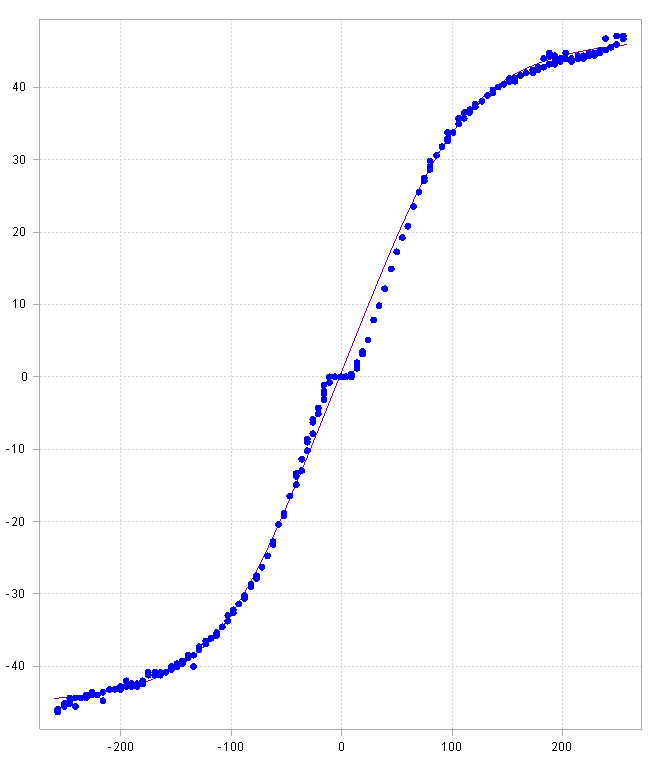
\includegraphics[width=0.75\textwidth]{Neuro}
                        \small Данные в виде точек и линия-обобщение. По оси Х располагаются сигналы, по оси У -- скорости
                \end{center}
                
                Особенность в районе нуля обусловлена наличием в системе трения и, чтобы "сорвать" систему из состояния покоя, требуется достаточно высокий момент вращения, который требует достаточно высокого сигнала на двигателях.
            \section{Результат подхода}

                На практике такой подход показывает себя плохо: поскольку сценарий обучения не соответствует сценарию использования. При управлении платформой скорость двигателей меняется достаточно часто(до двадцати раз в секунду) в достаточно широком диапазоне. Но функция регрессии спроектирована так, что желаемая скорость достигается через некоторое неопределённое время после выставления сигнала. Экспериментально установлено, что в среднем это несколько секунд. При динамическом управлении платформой это неприемлемый результат. Особенно заметна эта особенность при торможении.

                Более того, видно, что особенность вокруг нуля нейронная сеть не выучила. Эту особенность удалось выучить только разбиением пространства на 2: $Sig>0$ и $Sig<=0$ с независимым обучением двух сетей на этих пространствах.
            \section{Попытки модификации подхода к формированию экспериментальной выборки}
                Для приведения в соответствие сценария использования и сценария обучения была сделана модификация сценария сбора данных. Изменение: не ждать момента установления скорости вала и добавлять в выборку все пары ($Sig_l$, $Spd_c$). Этот путь тоже не приводит к нужному результату, поскольку выборка становится противоречивой и обилие информации нейронная сеть воспринимает как шум. В результате использование этой функции регрессии для управления двигателем ни в каких сценариях не даёт приемлемого результата.
            \section{Bывод}
                Прямой подход не даёт пригодного к использованию результата. Главным образом из-за того, что сеть не имеет достаточной информации для выдачи сигнала, подходящего к текущей ситуации. Например ситуации ускорения, торможения и равномерного движения требуют различного подхода к формированию сигнала: завышение, занижения и непосредственное соответствие. В том числе у сети нет временных рамок достижения скорости по сигналу, что даёт непредсказуемое время приведения системы в необходимое состояние. Таким образом мы получили список недостатков:
                \begin{itemize}
                  \item Отсутствие временных рамок
                  \item Отсутствие контекста применения сигнала
                      \begin{itemize}
                        \item Режим езды: ускорение, торможение, равномерное движение
                        \item Предыдущий выставленный сигнал индуцирует в катушке двигателя ток, который тоже нужно преодолеть
                      \end{itemize}
                  \item Сложная особенность в районе нуля
                \end{itemize}
                Все перечисленные проблемы решаются рассмотрением двигателя в терминах управляемых систем. Для управления двигателем в терминах системы введём понятие регулятора и цикла регуляции.
    \chapter{Инверсный нейрорегулятор}
        \section{Описание принципа устройства регулятора}
            Регулятор -- это сущность, которая способна вычислять управляющее воздействие для поддержания управляемой системы в указанном состоянии.
            Мы будем использовать термин регулятор в следующем ключе: регулятор -- это функция, принимающая три вектора:
            {
                \begin{enumerate}
                      \item \(\mathbb{S}_n,\, \mathbb{S}_n \in \mathbb{STATES}\),
                        вектор, описывающий состояние, которое необходимо поддерживать
                      \item \(\mathbb{S}_c,\, \mathbb{S}_c \in \mathbb{STATES}\),
                        вектор, описывающий текущее состояние управляемой системы
                      \item \(\mathbb{C}_l,\, \mathbb{C}_l \in \mathbb{CONTROLS}\),
                        вектор, описывающий прошлые управляющие воздействия, оказанные на систему
                \end{enumerate}
            }
            и возвращающая управляющее воздействие, которое приближает(не отдаляет) систему от целевого состояния \(\mathbb{C}_c,\, \mathbb{C}_c \in \mathbb{CONTROLS}\).

            В результате получим отображение, которое будем называть функцией регулятора.
            \[F:\,\mathbb{STATES}\times\mathbb{STATES}\times\mathbb{CONTROLS}\,\rightarrow\,\mathbb{CONTROLS}\]
            \[F(\mathbb{S}_n,\mathbb{S}_c,\mathbb{C}_l) = \mathbb{C}_c\]

        \section{Описание принципа устройства цикла регуляции}
            Предположим, у нас есть функция-регулятор. Цикл регуляции является бесконечным(не имеет выхода), каждый установленный промежуток времени $\Delta t$ снимаются показания состояния управляемой системы $\mathbb{S}_c$, формируется входная матрица для функции-регулятора $(\mathbb{S}_n,\mathbb{S}_c,\mathbb{C}_l)$, передаётся функции регулятору $F(\mathbb{S}_n,\mathbb{S}_c,\mathbb{C}_l)$, получаем управляющее воздействие $ \mathbb{C}_c$, применяем его к управляемой системе, продолжаем собирать данные о состоянии управляемой системы, пока через $\Delta t$ не нужно будет опять начинать цикл.

            Важной здесь является идея периодической корректировки управляющего воздействия: даже если состояние, в котором нужно поддерживать управляемую систему не изменится(не поступит новых команд), могут изменится параметры внешней среды, которые, если оставить их без реакции, могут сместить управляемую систему в нежелательное состояние. В том числе, периодичность полезна в том случае, если за одно управляющее воздействие невозможно привести систему в желаемое состояние (например из-за ограничений в максимальном ускорении, или из-за принципиальной неспособности контролируемого объекта менять состояния с требуемой скоростью). Как раз второе преимущество мы и будем эксплуатировать в дальнейшем.
        \section{Модель данных для случая управления двигателем}
            Зададим пространства состояний и управляющих воздействий для рассматриваемого случая.
            \[\mathbb{CONTROLS} = \mathbb{SIG};\, \mathbb{STATES} = \mathbb{SPD}\]
            То есть функция регулятор принимает вектор-строку в качестве аргумента и возвращает скаляр в качестве результата.
            \[F:\,\mathbb{SPD}\times\mathbb{SPD}\times\mathbb{SIG}\,\rightarrow\,\mathbb{SIG}\]
            \[F({Spd}_n,{Spd}_c,{Sig}_l) = {Sig}_c\]
        \section{Нейронная сеть в качестве функции-регулятора}
            \subsection{Формирование обучающей выборки}
                Для построения цикла регуляции нам нужна функция-регулятор. Применим ту же нейронную сеть для регрессии. Для проведения регрессии нужно собрать обучающую выборку. Причем обучающая выборка должна быть собрана в близких к сценарию использования условиях. Для сбора таких данных используем режим ручного управления с плавным изменением сигналов на колёсах. Выборка будет пополнятся, пока оператор платформы на ручном управлении совершает типичный для платформы манёвр. В выборке будут регистрироваться четвёрки
                    \[({Spd}_n,{Spd}_c,{Sig}_l,{Sig}_c)\]
                    \begin{center}
                      \({Spd}_n\) -- скорость в текущий момент времени\\
                      \({Spd}_c\) -- скорость в предыдущий момент времени\\
                      \({Sig}_l\) -- сигнал, приведший к предыдущей скорости\\
                      \({Sig}_c\) -- сигнал, приведший к текущей скорости\\
                    \end{center}
                Причем обязательным будет соблюдение цикличности: каждая новая выборка добавляется раз в $\Delta t$.
                Согласно правилам обучения сетей, подобных нашей, обучающая выборка перемешана и поделена на непосредственно обучающую и экзаменационную, на которой проверяются все необходимые метрики, являющиеся индикатором качества обучения.
                
                \begin{center}
                        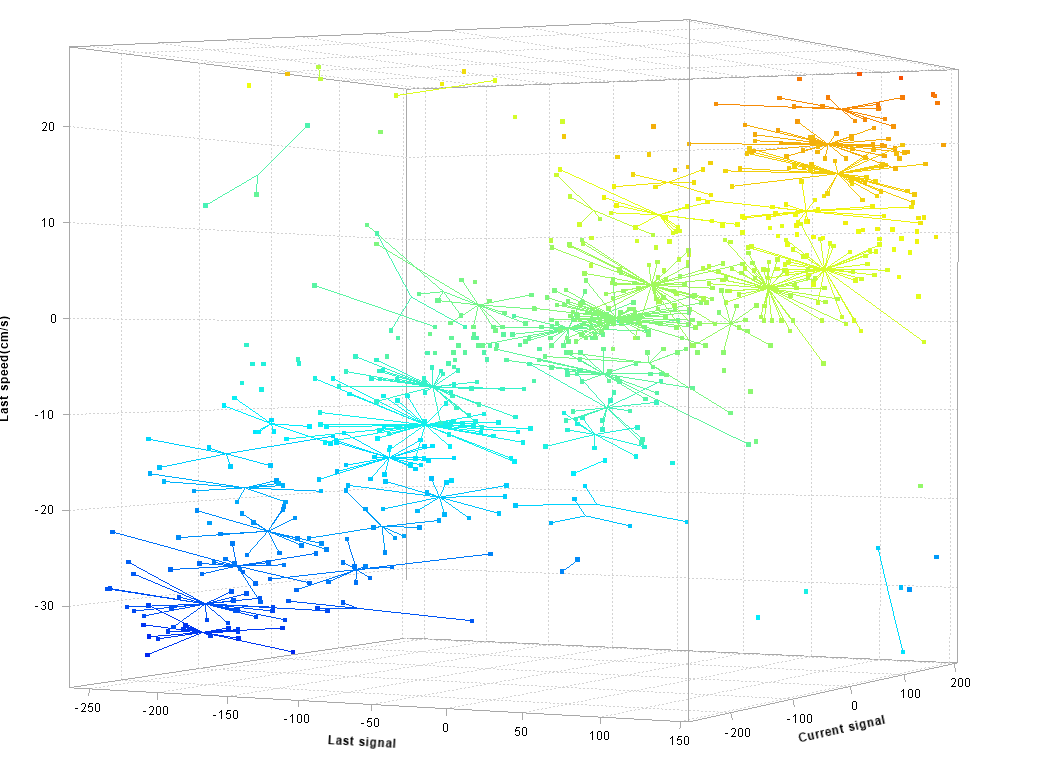
\includegraphics[width=0.85\textwidth]{clust1}
                        \smallОбщий вид четырёхмерного пространства. Желаемая скорость задана цветом. Пространство разбито на кластеры по принципу близости.
                \end{center}
                
            \subsection{Процесс обучения с учетом семантических ограничений}
                Поскольку в процессе обучения известна семантика зависимости, которую мы регрессируем, возникает желание учитывать ограничения и особенности предметной области при автоматическом обучении для достижения лучших результатов в типичных сценариях использования.

                Для того, чтобы появилась возможность учитывать особенности предметной области введём соответствующий механизм. Назовём этот механизм методом характеристик.
                Характеристика -- это просто функция, которая описывает какую-либо особенность поведения искомой функции в условиях, близким к реальным, и способна проверять наличие этих особенностей.
                В сущности, метод крайне прост: мы имеем список характеристик, на каждой итерации обучения сети проводится проверка, все ли необходимые характеристики наблюдаются и, если это так, нейронная сеть добавляется в список пригодных. Через какое-то достаточно большое количество итераций, например, когда в списке будет более десяти пригодных сетей, обучение останавливается и среди пригодных сетей выбирается та, которая имеет наиболее подходящий набор характеристик. Наиболее подходящая сеть выбирается оператором. Список характеристик выбирает также оператор исходя из текущих требований к поведению системы.
                Для улучшения качества обучения применили фичи: лавина, замыкание по нулю, среднее отклонение.

                Список наиболее хорошо показавших себя характеристик:
                    \begin{itemize}
                      \item Смещение средней ошибки от нуля. От результата выдачи сети на обучающей выборке считается средняя ошибка(не среднеквадратичная). Требуется, чтобы смещение не превышало единицы. В терминах предметной области, это значит, что сигналы, выдаваемые нейронной сетью отличаются от сигналов в выборке не более, чем на один. Напомним, что сигналы это $\mathbb{SIG} = \{Sig \in \mathbb{N}\,\vert -256 < Sig < 256\}$.
                      \item Точка "срыва". Стоит вспомнить особенность: в некой окрестности нуля по шкале сигналов, платформа не может сдвинуться с места из-за недостатка момента вращения на двигателях. В начале обучения эта характеристика вычисляет по обучающей выборке точку срыва следующим образом: точка срыва -- это средний сигнал из сигналов, которые перевели скорость колеса из нулевой в ненулевую за один цикл(\(\Delta t\)). На каждой итерации обучения проверяется, что сеть способна меньше чем за 5 циклов привести скорость колеса к ненулевой, если сети заказали $\frac{1}{100}$ от максимальной скорости колеса. Для проверки этой характеристики эмулируются циклы управления и проверяется, что на каком-то шаге ($<5$) выдача сети превышает точку срыва.
                      \item Замыкание вокруг нуля. Характеристика описывает следующее ожидаемое поведение: при заказе нулевой скорости, если текущая скорость околонулевая, должен выдаваться околонулевой сигнал. Это очень важная характеристика, она требует, чтобы сеть не могла достигнуть точки срыва из состояния, близкого к покою, если от неё не требуют движения. Кроме того, что характеристика гарантирует отсутствие движения, если оно не требуется, её наличие существенно улучшает поведение сети на всём пространстве. Существует гипотеза, что эта характеристика гарантирует робастность функции-регулятора, однако простого доказательства этому факту не нашлось. Характеристика проверяется подобно характеристике о точке срыва: эмулируются циклы регуляции, цикл начинается с параметрами, соответствующими покою и ненулевому сигналу на предыдущем шаге цикла. Проверяется уменьшение сигнала с каждым шагом цикла регуляции.
                    \end{itemize}
                
                \begin{center}
                        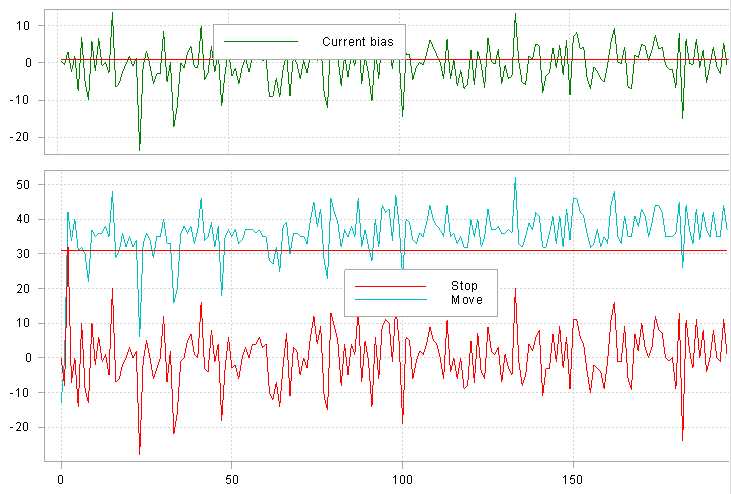
\includegraphics[width=0.85\textwidth]{Features}
                        \smallЗначение характеристик во время обучения. По оси Х отложены номера итераций обучения.
                \end{center}
                    
                Все остальные характеристики сильно коррелировали с указанными и перестали использоваться, как менее информативные и менее поддающиеся интерпретации с точки зрения предметной области. Среди них средневкадратичное отклонение, мера объяснённости эксперимента, требования монотонности по переменным.
                Также была сделана попытка добавить следующий критерий: различие метрик сети на экзаменационной выборке и на обучающей не должны быть статистически значимы. Однако этот подход детектировал не качество самой сети, а наличие классических ошибок при обучении сети: паралич сети, переобучение. Поскольку такие ошибки не проявлялись, от поддержки метода отказались.
                
                
        \section{Результат}
                \begin{center}
                        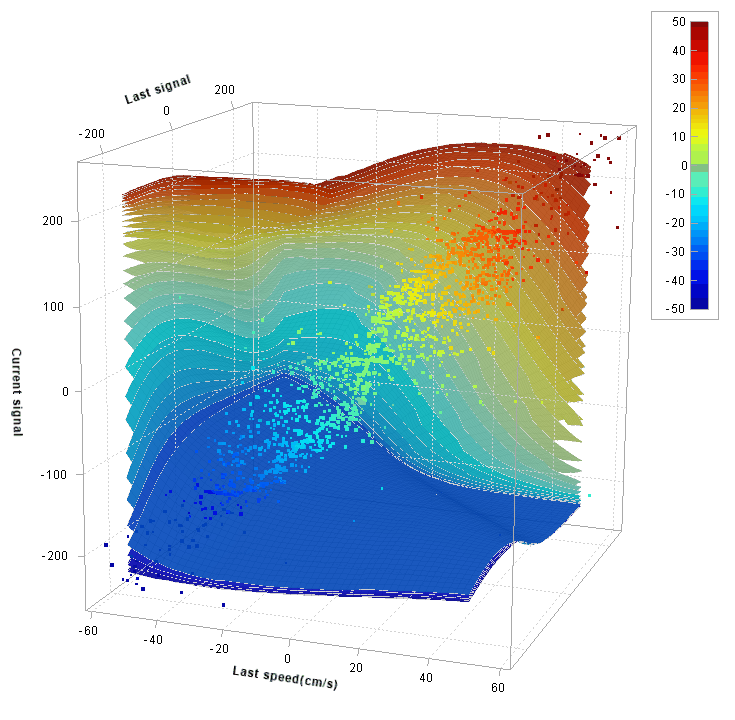
\includegraphics[width=0.85\textwidth]{surface}
                        \smallОбщий вид гиперповерхности нейронной сети.
                \end{center}
        
            Результирующая функция регулятор выполняет все поставленные задачи и даже имеет несколько неожиданных, но крайне удобных свойств.

            Среди поставленных задач:
                \begin{itemize}
                  \item Предсказуемая динамика изменения скорости. На практике сеть выдаёт сигнал так, что ускорение в пределах цикла регуляции можно считать равномерным.
                  \item Мягкое ограничение максимального ускорения. За счет циклической природы управляющего алгоритма сеть может не выдавать сигнал, приводящий к чрезмерному ускорению, но при этом всё равно выполнять задачу контроля скорости.
                  \item Активное торможение. Сеть получила способность выдавать инверсный сигнал для торможения. В случаях, когда сети нужно достаточно быстро сбросить скорость, она выдают сигнал, противоположный текущему, но при этом такой, чтобы ускорение колеса было не слишком велико. Это свойство придаёт платформе очень хорошие динамические характеристики движения.
                \end{itemize}
            Неожиданные полезные свойства:
                \begin{itemize}
                  \item Способность увеличивать сигнал, если момента силы на колесе недостаточно для достижения заказанной скорости. Например, даже если заказать крайне низкую скорость и не позволять колесу свободно вращаться, то двигатель очень быстро выйдет на предельную мощность. На практике это позволяет переезжать препятствия без изменения скорости колеса.
                  \item Независимость качества управления от заряда аккумулятора, питающего двигатель. Поскольку сигнал выдаваемый на двигатели фактически является лишь делителем напряжения, поступающего с аккумулятора, ожидалось, что при значительном изменении напряжения аккумулятора от значения, при котором сеть калибровали, динамические характеристики будут непредсказуемо меняться, поскольку зависимость момента силы от напряжения далека от линейной. Однако этого не произошло и сеть была способна управлять двигателями даже при 30\% разнице значений.
                \end{itemize}

            Как показала практика, параметры сети не влияют на качество работы регулятора. Фактически, подходят любые не экстремальные параметры. Приведу конфигурацию сети, которая использовалась при написании дипломной работы:
                \begin{center}
                  Функция активации(Activation function): биполярная сигмоида\\
                  Параметр функции активации(Activation fuction parameter): 2.2\\
                  Момент(Momentum): 0.7\\
                  Скорость(Rate): 0.3\\
                  Топология сети(Layers configuration): 3, 7, 3, 1
                \end{center}
        \section{Вывод}
            Поскольку результирующее поведение системы крайне похоже на поведение системы, управляемой хорошо спроектированным регулятором, результаты интерпретируются достаточно однозначно: нейронная сеть выучила робастную функцию-регулятор. Фактически описанная техника позволяет управлять широким спектром устройств без знания природы процессов внутри контролируемых систем, которые были бы необходимы для проектирования классических регуляторов.
    \chapter{Калибровка инфракрасных дальномеров}
        \section{Постановка задачи}
        \section{Описание реальных характеристик дальномеров}
        \section{Модель данных}
        \section{Процесс обучения сети}
        \section{Сглаживание оригинала}
        \section{Результат}
        \section{Вывод}

\newpage
    %\chapter{Список литературы}
        \begin{thebibliography}{99}
        %\addcontentsline{toc}{section}{Литература}
            \bibitem{OmatuKhalidUsuoph} Омату С., Халид М. Юсоф Р. {\it Нейроуправление и его приложения} // Издательтво $"$ИПРЖР$"$, 2000.
            \bibitem{Galushkin} Галушкин А.И. {\it Нейронные сети. Основы теории} // Издательство $"$Горячая Линия - Телеком$"$, 2012.
            \bibitem{Khaykin} Хайкин С. {\it Нейронные сети. Полный курс} // Издательство $"$Вильямс$"$, 2006.
            \bibitem{Uorssermen} Уоссермен Ф. {\it Нейрокомпьютерная техника: Теория и практика} // Издательство $"$Мир$"$, 2006.
        \end{thebibliography}

\end{document} 